
\chapter{Introduction}
\label{c-intro}

In this chapter, we survey the area and lay conceptual foundations for the rest of the paper. We first provide an overview of different approaches to IR evaluation. We then focus on offline evaluation, explaining traditional approaches and recent trends. Finally, we introduce a conceptual framework and the outline for the rest of this paper.

\section{Evaluation Paradigms in IR}
\label{sec:evaluation-paradigms}

Evaluating a search system, or any system that supports information access such as recommendation or filtering, is a complex problem. The performance of a search system is dependent on various contextual factors, such as the task at hand, the user's preference, abilities, location and other characteristics, and even the timing of the interaction. Also, the ultimate source of ground truth, the user's judgment, is subjective, volatile, and often hard to come by.

\subsection{Offline vs. Online Evaluation}

In order to meet these challenges, IR researchers have built a rich evaluation tradition. Most of this work has been based on a few simplifying assumptions. The document collection is static and the user's information need is represented as a description or a keyword query. The user's judgments in situ are replaced with judgments collected post-hoc and from third parties, often in the form of binary or numeric-scale labels.

We can define this evaluation paradigm as \textit{offline evaluation} \citep{INR-009} in that the evaluation of the system can happen without requiring an actual user. This makes offline evaluation particularly suitable for early-stage evaluation of an IR system, when users are hard to come by. Another typical characteristic of offline evaluation is that the test collection (a set of tasks, judgments and documents) is 'reusable', in that once built it can be used to evaluate new systems; because many factors are controlled, evaluations are also commensurable across time and between researchers.

An evaluation paradigm contrasting with offline evaluation is called \textit{online evaluation}. In a recent survey on this topic, online evaluation is defined as the evaluation of a fully functioning system based on measurement of real users' interactions with the system in a natural environment \citep{INR-XYZ}. That is, online evaluation directly employs user behavior in natural environment for evaluation.

As large-scale online services become commonplace, online evaluation becomes a viable option for companies with running services with large user bases. In the literature, there has been a plethora of papers on methodologies for online evaluation. While online evaluation has benefits in using data readily available as a by-product of serving users, this dependence on user behavior also creates limitations for online evaluation, which we will discuss later in this section.

\subsection{Hybrid Approaches}

So far we have introduced two evaluation paradigms -- offline and online evaluation -- with distinctive characteristics. Offline evaluation is based on human judges as substitution of real users, and has strengths in experimental control and reusability. Online evaluation is based on user behavior, and has strengths in fidelity and cost.

% \paul{really? How about ``\dots is based on abstractions of real users''?}

While these two approaches comprise the majority of evaluation efforts, there have been several approaches trying to find a middle ground. Click modeling \citep{chuklin2015click} and counterfactual online evaluation \citep{Li:2015, li2010contextual}, for example, re-use online user data for future evaluation. These approaches, while enabling the re-use of online user data, are still limited in that they are based on implicit signals from user behavior. For instance, it is not possible to decide with certainty whether a user indeed found the clicked document relevant or not, even with all the contextual information.

%\paul{how is that a limitation? need to be explicit}\jin{I tried to explain}

Another related line of work is user study-based evaluation \citep{Bron:2013, Liu:2014, Shah:2011}, which is widely used in interactive IR studies \citep{kelly2009methods}. In such work, a group of participants are typically brought into a lab environment and asked to perform a set of (usually predetermined) search tasks. It is common for this type of study to collect both behavior and labels from the participants to get a more complete picture of search activity. 

User studies bear similarities with offline evaluation in that they typically involve some form of explicit judgments, but their emphasis is more on understanding some aspect of users' search behavior, as opposed to comparative evaluation among search systems. Also, user studies tend to be limited in scale (typically less than 100 participants) and based on a biased, possibly not representative, sample of participants (typically people within the same institution).

However, the distinctions are getting blurred as search engines increasingly serve more complex results, and SERP (search engine results page) or session-level evaluation is drawing more attention. In fact, some recent research has tried to use task completion settings for system-to-system comparison \citep{Xu:2009}. Also, crowdsourcing techniques are reducing barriers in getting access to a large number of subjects with diverse backgrounds. We will return to this point in Chapter~\ref{c-human-judgment}.

\subsection{When to Use Offline Evaluation}

\begin{figure}
	\centering
	{
	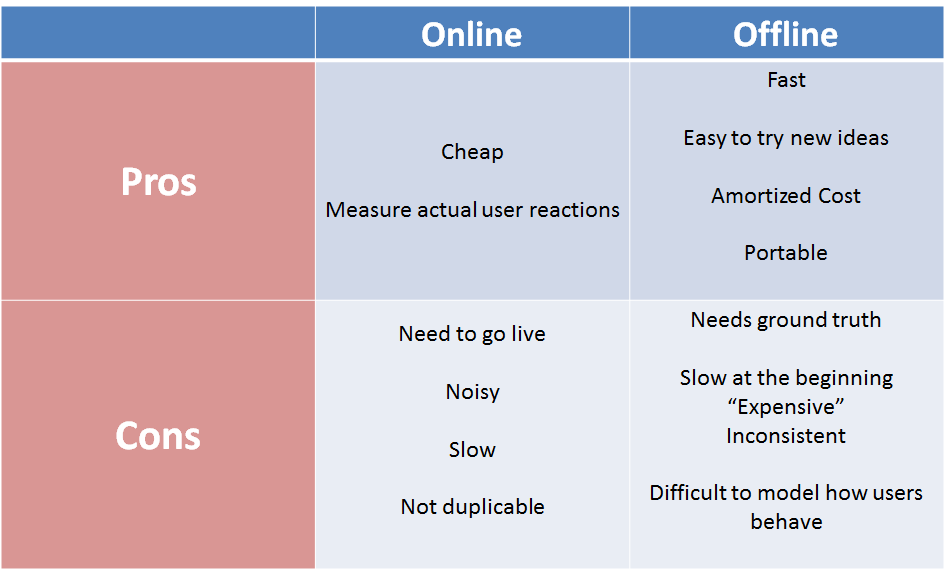
\includegraphics[width=0.9\textwidth]{images/online_vs_offline}
	}\vspace*{3em}
	\caption{Pros and cons of offline vs. online evaluation}
\end{figure}\label{onlinevsoffline}
\paul{Figure~\ref{onlinevsoffline}---perhaps retype? The screen grab is pixellated. Also NB capitals in ``Cost/Reusability''}

At this point, a reader may ask: when should we use online vs. offline evaluation? While online metrics are certainly valuable and must-have when feasible, there are reasons we may need explicit input from human judges. 

Figure~\ref{onlinevsoffline} summarizes the advantages and disadvantages of online vs. offline evaluation. Offline evaluation typically requires access to explicit judgments of relevance obtained from relevance assessors, or judges. Obtaining judgments is an expensive procedure; hence, online evaluation tends to be cheaper compared to offline evaluation. Furthermore, online evaluation is based on signals that directly come from real users, which can enable us to get a more realistic signal of user satisfaction. 

On the other hand, online evaluation requires a running system as it is based on signals from real users. First, in initial stages of system development we simply might not have real users to study. Furthermore, small companies and academics may not have access to a large volume of users to be able to collect reliable signals. On the other hand, with the availability of various crowdsourcing services, it is relatively easy to collect labels from human judges.

Another major problem in online evaluation is that usually a significant amount of usage data is needed before one can reach reliable signals of satisfaction. Hence, online evaluation tends to be very slow, which may not be suitable for evaluating the quality of new methodologies quickly. On top of this, online evaluation necessitates the maintenance of a production system with a large user base along with experimental infrastructure, which is possible for large corporations but challenging otherwise.

More importantly, signals obtained from real users tend to be noisy and traces of user behavior are often insufficient to measure a user's true satisfaction. As an example, let's take clicks on results for evaluating a search engine. While a click is certainly an indication that the user is interested in the result, it is not clear whether the clicked result was actually satisfying. Also, clicks are often concentrated on the top of the page regardless of result quality, making them difficult to interpret. That is, the ambiguity and bias inherent in user behavior often make it hard to infer the true quality of our products. 

Another consideration is the reusability of the data collected. In offline evaluation, typically the label is collected at the level of individual information item (i.e., document) and the system is evaluated by its ability to put more relevant items on top. This means the labels can be reused to evaluate new systems that produce different rankings of the same items. By contrast, the data collected from online system is only valid for the evaluation of the system user interacted with, and the data should be collected for every new system to be developed.

Offline evaluation, on the other hand, tends to be fast once explicit judgments of relevance are obtained from relevance assessors. Once these judgments are collected, they can be used to evaluate the quality of sytems quickly. This makes offline evaluation very suitable for trying new ideas, and the initial cost can be amortised over many experiments. Furthermore, offline evaluation mechanisms can be used to evaluate the quality of new systems; hence, they tend to be reusable and portable.

One major drawback of offline evaluation is the expense of collecting these explicit judgments, or the ground truth. Obtaining relevance judgments tends to be quite slow and expensive. Furthermore, these explicit judgments of relevance tends to come from a third-party assessor, as opposed to the real user of the system. Hence, the assessor may have a different understanding than an actual user as to what documents should be considered relevant. Furthermore, different relevance assessors can also disagree with each other, leading to inconsistencies in judgments. 

Finally, offline evaluation metrics tend to be based on \emph{models} of user behavior, as opposed to behavior signals obtained from real users and modeling users can be quite challenging due to the variance in behavior and expectations of real users. Hence, evaluation metrics based on user models may not necessarily reflect user satisfaction. Much recent work in offline evaluation focuses on this issue, which we will review later this paper.\paul{where? need ref}

Given these advantages and disadvantages associated with online and offline evaluation, it is no wonder that most large scale companies tend to use a combination of both mechanisms. Offline evaluation mechanisms tend to be used for quickly measuring the quality of new methods, and algorithms that show promising results are deployed to some selected subset of real users. Online evaluation mechanisms are then used to make the final decision about full-scale deployment. On the other hand, among smaller companies with limited users, and among academic researchers, offline evaluation remains the only feasible mechanism. 

\section{Offline Evaluation for IR}

Information retrieval has a rich tradition of evaluation, both online and offline, and this tradition has been responsible for some of the rapid advances in search technology of the past two decades~\citep{TRECimpact}. Below we survey traditional approaches to offline evaluation, and consider trends in recent years which suggest new roles and methods.

\subsection{Traditional Approaches to Offline Evaluation}

The traditional offline approach to IR evaluation is the test collection, or ``Cranfield'', approach first described by \cite{cleverdon67} and refined through exercises such as the Text REtrieval Conference (TREC; see \cite{voor:trec05} for an overview).  We will summarise this approach here, noting that \cite{INR-009} provides a historical summary and comprehensive discussion.

\begin{figure}
	%\centering
	{
	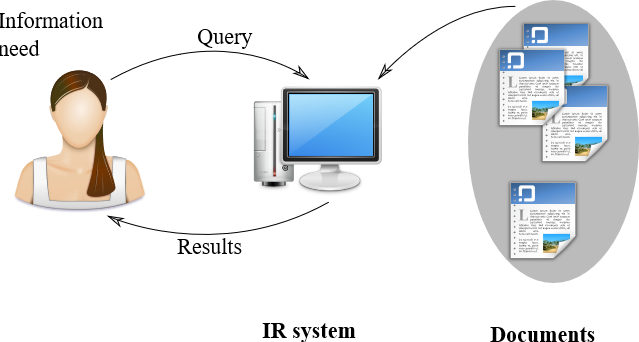
\includegraphics[width=0.67\textwidth]{images/ir-model}
	\subcaption{A simplified model of a retrieval system in context.}
	\label{fig:ir-simple}
	}\vspace*{3em}
	{
	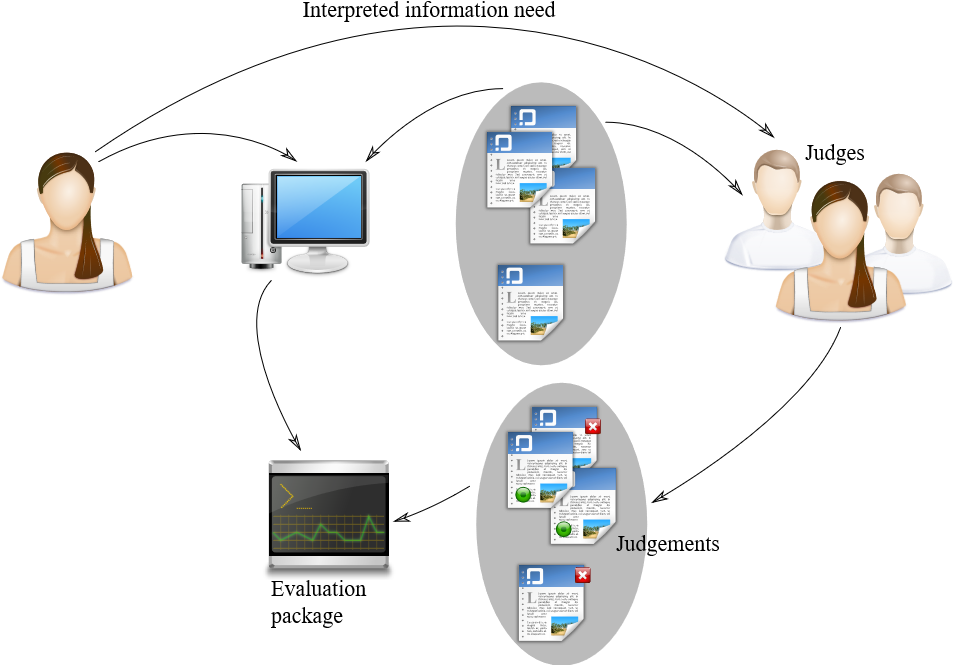
\includegraphics[width=\textwidth]{images/ir-model-with-judges}
	\subcaption{Extension of the model, illustrating third-party relevance judges and the formation of a test collection.}
	\label{fig:ir-with-judges}
	}\vspace*{3em}
	\caption{Test-collection-based evaluation of an information retrieval system.}
\end{figure}

In its most basic form, we can think of an information retrieval system as mediating access to a collection of documents. A user has an information need; they express this as a query; and the system will draw on the document collection to produce some set of results (Figure~\ref{fig:ir-simple}).

The test collection approach simulates this model by using judgements of relevance and evaluation metrics that aim at measuring the quality of the results presented to the user  (Figure~\ref{fig:ir-with-judges}). The query, document collection, and retrieval system are as before but three components are added:

\begin{description}
	\item[Judges] interpret the user's information need, for example on the basis of the query or other context; and consider the extent to which each document in the collection answers this need.
	
	\item[Judgments] record this information obtained from the judges for each (query, document) pair.
	
	\item[Evaluation] is then a matter of aggregating the recorded judgements for the set (or ranking) of documents retrieved by the system; or comparing the documents retrieved with the documents judged as relevant.
\end{description}

For example, precision can be calculated by counting the number of retrieved documents which were marked as relevant; recall can be calculated by comparing the number of retrieved documents judged relevant with the overall number judged relevant; or rank-sensitive metrics, such as average precision or reciprocal rank, can look at the judgment for each retrieved document in turn.

\subsubsection{Abstractions}

In principle, the judgements formed are complete---that is, the collection includes a judgment for each possible (query, document) pair. Although this was true of some of the earliest exercises, \paul{need ref for Cranfield II, which I believe was complete} it is clearly impossible for today's much larger document sets. Two shortcuts have allowed researchers to collect useful judgments regardless.  First, a simplifying assumption is that every search is over the same, fixed, document collection: that is, the documents do not change over time and nor are they different for different information needs (or users---as would be the case for personal or corporate collections).

Even allowing for this, it is clearly impossible to judge each of millions (or billions) of documents for any arbitrary information need. \emph{Pooling} provides a common shortcut. In a pooled evaluation, each of a number of search systems provides its own ranking of documents, perhaps by running the same query on each. Every document which appears in the top~$k$ in any ranking is then judged, so if $N$~systems contribute to the pool there are at most $Nk$~judgments to be made: likely fewer, as some documents will appear in more than one list.

A related assumption is that each need can be captured in a single expression: that is, most (although not all) collections include a single query for each need.  Although this is clearly a very small sample of possible inputs for the need, and although relatively small changes to a query can result in large changes in measured effectiveness~\citep{bailey15user}, a large sample of needs can still capture useful variation.

Judging is also abstracted from real users in real contexts, in order to collect judgments at scale. The largest assumption here---indeed, an assumption relied upon by most effectiveness metrics---is that judgments are independent. That is, it is assumed that the extent to which a document is relevant to a need is independent of any other document which might be returned, or the order in which they are seen by the user. Notable exceptions are techniques from \cite{Golbus:2014} and \cite{CDR,Chandar2013}, who used relevance judgments based on other documents.

The notion of ``relevance'' is also normally abstracted. Although in reality relevance is complex, multi-facteted, and highly contextual \citep{borlund2003,saracevic16relevance}, judges are often given much simpler instructions which can for example boil down to what \cite{borlund2003} calls ``intellectual topicality'' alone. Recent work such as that by \cite{Mao:2016} and \cite{VermaYC16} also aims at extending this narrow definition of relevance. We delve into this in Chapter~\ref{c-human-judgment}.

\subsubsection{Test Collections and TREC}

A central concept in traditional IR evaluation is the \emph{test collection}. A test collection is the combination of 

\begin{itemize}
	\item a fixed set of documents; 
	\item a set of information needs or topics, typically each with an associated query; and 
	\item a set of relevance judgments which detail the relevance of at least some documents to each need.
\end{itemize}

Because they involve a static representation of an information-seeking session, test collections can be distributed; the judgments therein are reusable; and, in combination with one or more effectiveness metrics, they make it simple to compare systems.

%\subsubsection{Building Collections}
%
%\paul{to do?} glossed over the many questions of how to build these in practice. simulated work tasks. query variation. pooling choices. labelling choices, judge selection (g/s/b). etc. see\dots

%\subsubsection{Shared Evaluation Exercises}

Test collections have been especially valuable for evaluation as they are easy to re-use: typically the limiting factor is just physical (or network) distribution of the documents themselves. Since they are so abstracted, they are self-contained, and it is trivial to compare results across systems, times, or laboratories.

A noteworthy example of this is the Text REtrieval Conference (TREC) series, run annually by the (U.S.) National Institute of Standards and Technology (NIST). Since 1992 these conferences have been based around shared evaluations, using test collections so that each participating system can be directly compared to others~\cite{voor:trec05}. The model has been adopted by a number of other conferences \paul{refs}. These collections now include genera such as the web, microblogs, genomics, tourism, email, and others and in virtue of their scope and portability have become standard tools for information retrieval research.

\subsection{Recent Trends in Offline Evaluation}

So far we have looked at traditional approaches in IR evaluation. While this tradition has served the community well for the past few decades, there has been several trends which necessitate a change in the roles and methods of IR evaluation. In this section, we outline recent trends and discuss implications for offline evaluation.

\subsubsection{User-Centric Evaluation}
First and foremost, online search engines with large-scale user bases have become commonplace, enabling online evaluation based on user behavior. This availability of user data has opened up the possibility of validating the assumptions of offline evaluation with actual user data. Recent work on evaluation metrics has embraced online user data to tune parameters of the metrics \citep{CarteretteKY11, Carterette:2012}.\paul{add ref to time-biased gain, which uses online data on reading times; cascade model etc, which uses P(click)}

The overall outcome of this trend is the advent of new IR evaluation paradigms which are more user-centric, diverse and agile. Here, being user-centric means that the evaluation process is based on a model of user behavior, or/and aims to improve user satisfaction or other user-visible measure such as engagement or task completion \citep{scholer13}. 

This has already led to new methodologies to better estimate user satisfaction and behavior in judgment collection \citep{VermaY16, VermaYC16} or metric design \citep{YilmazSCR10, CarteretteKY11, ChapelleMZG09}. Also, some recent work has looked at cross-metric correlation, aiming to align IR evaluation with user satisfaction or some proxy of it \citep{Al-Maskari2007,radl:comp10}.

%As a side note, there has been an increasing efforts to combine online and offline evaluation. These include ways to use online user data for offline evaluation \cite{Li:2015} \cite{li2010contextual} \cite{chuklin2015click}, or ways to collect feedback directly from user \cite{Kim2016}. 
%\note{mentions of user study / iir papers}

\subsubsection{Diverse Endpoints and Search Scenarios}

There are also new endpoints for search beyond desktop web browsers, such as mobile phones and conversational agents. This has opened up a whole area of research which focuses on different interaction methods and user experiences across endpoints. For instance, mobile devices have much smaller screen dimensions and the interaction is based on touch, while conversational agents use natural language, often in voice, to interact with the user.

Even for web search itself, the types of search results have diversified beyond the list of web documents to include other results types such as images, videos, news and even direct answers. This diverse set of results types, and corresponding user interface designs, breaks many assumptions of traditional IR evaluation, providing rich opportunities for exploration. In particular, many of these 'answers' can directly satisfy users' information needs on the SERP, making it hard to apply click-based evaluation techniques \citep{Li2009GA,diriye2012leaving}.

IR evaluation research has responded to this needs with various lines of work. There has been increased interest in whole-page evaluation and optimization \citep{Zhou:2012}, which encompasses a wide variety of page elements beyond web results. %Side-by-side evaluation 
%
Task and session-level evaluation has also drawn interest \citep{KanoulasCCS11, CarteretteKHC14}, with TREC tracks of the same name \citep{carterette2014overview}. Finally, there have been new lines of work focusing specifically on mobile interfaces \citep{VermaYC16}, or evaluation of search with spoken agents \citep{Kiseleva:2016}.

\subsubsection{Crowdsourcing / Agile Evaluation}

These diverse new endpoints and scenarios for search required ways to collect labels in a more agile manner, because many of these services are new and exploratory by nature, with less investments compared to well-established ones like web search. Also, in academic settings, it has been difficult to recruit participants with diverse backgrounds at scale.

Fortunately, services such as Amazon Mechanical Turk have provided new ways for human judgments of any kind to be collected at an large scale. These services are called `crowdsourcing', in that they pull the `wisdom of the crowd' for tasks needing human intelligence. Accompanying this new data collection method is a challenge in quality control, since the labeling work is completed by a remote worker on the internet.

Given these opportunities and challenges, there has been quite a good deal of research on collecting high-quality labels with low effort \citep{Alonso2012}. Popular approaches include using overlapping judgments to identify ground truth labels \citep{Venanzi:2014}, or identifying the quality of judges based on their behaviors \citep{Kazai:2016}. We cover some of these methods in Section \ref{s-crowdsourcing}.

%\emine{Should we define that crowdsourcing is and how it may be useful for offline evaluation?}

\section{Scenarios for Offline Evaluation}

We have outlined basic concepts and recent trends for offline evaluation so far. The goal of this paper is to provide a practical guide to conducting offline evaluation for both academic and industry practitioners. Since there can be various scenarios in conducting offline evaluation, here we outline possible ones which we cover in this paper.

In classical IR research, a typical evaluation scenario is to improve the performance of a system given a test collection and a pre-determined set of evaluation metrics. For instance, in the TREC Web Track, participants are given a collection representative of the Web, and then asked to submit the results for their systems in a designated format. These are then evaluated on metrics like NDCG \citep{Jarvelin:2002} or ERR \citep{ChapelleMZG09}.

While academic IR research has developed well-accepted evaluation practices as above, the situation is a lot more ill-defined and varied from a practitioners' standpoint. There are multiple components in a modern IR system such as a web search engine, and each requires different emphases and considerations. For instance, one can think of component-level (i.e., query suggestion) evaluation as opposed to system-level evaluation. 

Also, building a working system serving real users takes several stages of development. The evaluation at early stages of development would be more exploratory in nature, whereas at later stage the focus would shift to making ship decisions. We can call the former \textit{information-centric} evaluation in that the goal is to collect information helpful for system development and debugging, where the latter can be considered \textit{number-centric} in that the goal is to get reliable performance numbers for decision making.\paul{we don't use these terms again anywhere}

Another characteristics of IR evaluation in industry settings is that the evaluation is an on-going process which takes multiple iterations over the lifetime of the service, as opposed to a one-off research project. This necessitates the development of so called \textit{evaluation pipelines} where any new system can be evaluated on a ongoing basis.

Since the goal of this paper is to meet the need of practitioners as well as academic researchers, we describe decisions one needs to face in conducting offline evaluation across various scenarios outlined above. We also focus on considerations in designing a evaluation pipeline in industry settings at Chapter~\ref{c-practice}.

\section{General Framework for Offline Evaluation}

In this section, we describe in detail a framework for offline evaluation. The goal is to propose a general framework which can encompass the diverse set of scenarios outlined above. 

\subsection{Definitions}

First, here are a few definitions that will be used throughout this paper. These comprise the components of offline evaluation.

\paragraph{Search Task} A search begins with user's information needs, which we call a search task. Search tasks can be represented as a description of these needs, or queries user would have used in actual information seeking.

\paragraph{Judging Target} Judging target denotes a result produced by an IR system, and the item which is evaluated. It can be of any granularity -- a snippet, a web document, or entire SERP. 

\paragraph{Human Judgment} A human judgment is an assessment of a \textit{judging target} by a human judge, in the context of a \textit{search task}, over some dimension of quality. 

\paragraph{Evaluation Metric} An evaluation metric (or metric in short) summarizes judgments into a single score. The design of an evaluation metric depends on the type of judgments being collected, and the model of user behavior.

\paragraph{Test Collection} A test collection is a collection of tasks, targets, and judgments with a specific evaluation goal. An evaluation metric summarizes the outcome of an experiment with a test coollection, and an appropriate statistical test can make a claim about the validity and reliability of the findings.

\subsection{Evaluation Process}
Given the components above, here we discuss the general process for offline evaluation. At a high level, offline evaluation is composed of three steps: 1) judgment design, 2) metric design and 3) experiment design. Alternatively, you can consider the whole process in terms of collecting data (judgments), combining them into meaningful numbers (metrics), build a test collection to drawing conclusions from (test collection). Now we discuss major considerations in each step.\paul{surely you need a collection, or at least 2/3 of it -- tasks and docs -- to get the judgements in the first place. Perhaps ``\dots, carry out experiments to test hypotheses and draw conclusions''?}

%\begin{figure}
%	\begin{center}
%		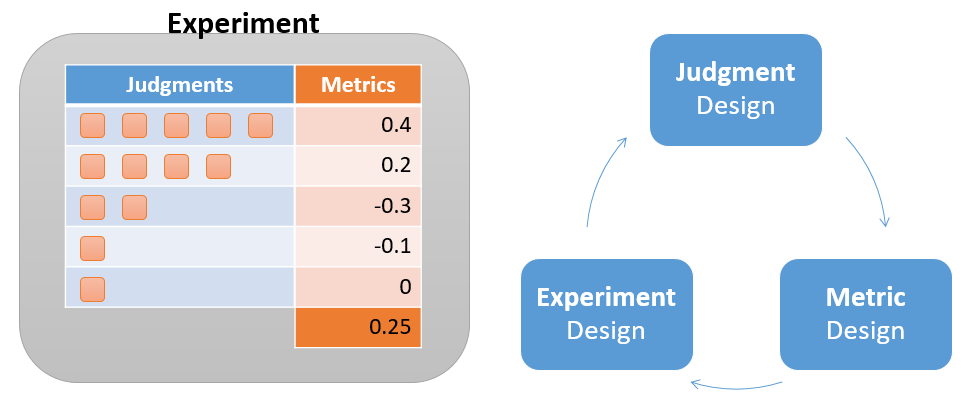
\includegraphics[scale=0.4]{images/offline_evaluation_overview}
%		\caption{Overview of Offline Evaluation.} 
%		\label{fig:offline_evaluation_overview}
%	\end{center}
%\end{figure}
%\emine{This figure shows as though the metric is part of the test collection so we might need to change that}
\subsubsection{Designing Human Judgments}

In the first step, the details of human judgment should be defined, which is the basic unit of offline evaluation. Human judgments capture the quality of the results for given search tasks. Here are major considerations in this step:

\begin{enumerate}
	\item How do you define and collect search tasks?
	\item What should be your judging unit?
	\item How do you design judging interface?
	\item How do you hire and train judges?\paul{we don't cover training in ch2}
\end{enumerate}

\subsubsection{Designing Evaluation Metrics}

The second step in offline evaluation is selecting or designing a  evaluation metric. Metrics summarize the information from individual labels into meaningful numbers. This is essentially the question of how to combine labels to meaningful numbers.

\begin{enumerate}
	\item How do you transform the labels from human judges?
	\item How do you define user models in combining labels into a metric?
	\item How do you estimate the parameters for the user model?
\end{enumerate}

\subsubsection{Designing Experiments}

\paul{was ``designing test collections'', please check you're happy with the re-wording}

Lastly, judgments and metrics should be combined to achieve the goal of evaluation. Since this is an iterative step which takes several stages of refinement, here we describe methods and criteria in doing so. 

\begin{enumerate}
	\item How do you size the test collection to fulfill your evaluation goal?
	\item How do you evaluate the validity of the outcome?
\end{enumerate}


\section{The Organization of this Paper}

In the following chapters, we describe each process of offline evaluation in detail so that a reader can design his or her own evaluation pipeline following the flow of this paper. Chapter~\ref{c-human-judgment} deals with gathering judgments, which need to be created for the purpose. Chapter~\ref{c-metric} considers steps in designing an effective metric. Chapter~\ref{c-collection} covers the methods in designing and analyzing experiments. Finally, Chapter~\ref{c-practice} describes evaluation practices from major companies in search and recommendation area.

%\emine{We already had a part describing the organization. In general, this section feels a bit repetitive given the text in first page}
%\paul{I disagree, that was in the abstract; it makes sense here (as well) I think. Unless I missed something?}